%Phone 
%open chapters on any page, final removes formatting marks
%avoid conflicts with hyperref by loading before documentclass
\RequirePackage{setspace}

\documentclass[11.75pt,openany,final]{memoir}
\makepagenote
\title{The Discoverer's Digest}
%place graphics package first to avoid conflicts (weird page sizes)
\usepackage{graphicx}
\usepackage{wrapfig}

% package to remove 'Figure x.x' with the \caption*{foo} option
\usepackage[labelformat=empty]{caption}

%\usepackage[paperwidth=70.9mm, paperheight=143.6mm, hmargin={1cm, 1cm},vmargin={1.2cm, 1.25cm}]{geometry}
% New setup
% setstocksize{height}{width}
\setstocksize{216mm}{137mm}
\settrimmedsize{216mm}{137mm}{*}
\settypeblocksize{216mm}{137mm}{*}
\setlrmarginsandblock{24.0mm}{24.0mm}{*}
\setulmarginsandblock{27mm}{27mm}{*}
%\marginparmargin{2mm}
% memoir: finalize the page changes
\checkandfixthelayout

\usepackage{microtype}

% \usepackage{marginnote}
%\usepackage{wrapfig}
%\setbeforesecskip{2mm}
% \setaftersecskip{2mm}
%\setSindent{0pt}

% TYPEFACE PROPERTIES
%--------------------
% fontspec system for typeface definitions
\usepackage{fontspec,xunicode,polyglossia}

%NOTE: good discussion of fonts: https://tex.stackexchange.com/questions/352804/setmainfont-vs-fontspec
%letter spacing

%fontspec font selection
\setmainfont{LinuxLibertineG}[
BoldFont = LinuxLibertineGB,
ItalicFont = LinuxLibertineGI,
BoldItalicFont = LinuxLibertineGZI,
SlantedFont = LinLibertineSlantedZ,
BoldSlantedFont = LinLibertineSlantedZ,
SmallCapsFont = LinLibertineCapitals
]
\setmonofont{LinLibertine_M}
\setsansfont{LiberationSans}


\makeatletter
%\g@addto@macro\chapnamefont{\sffamily} 
%\g@addto@macro\chapnumfont{\sffamily}  
%\g@addto@macro\chaptitlefont{\sffamily}
%\makeatother

% PAGE PROPERTIES
%----------------
%% common ligatures
%TODO: add more ligatures
\usepackage{newunicodechar}
\newunicodechar{ff}{ff}
\newunicodechar{fi}{fi}
\newunicodechar{fl}{fl}
\newunicodechar{ffi}{ffi}
\newunicodechar{ffl}{ffl}
%% end of common ligatures

% multiple columns (bullet lists, etc.)
\usepackage{multicol}

% set the leading
%better as it leaves margin note spacing alone
\setstretch{1.20}

%flexible margin notes
\usepackage{marginnote}
\renewcommand*{\marginfont}{\color{gray!80!black}\tiny\itshape\setstretch{0.9}}
% End notes
%\usepackage{enotez}
%\setenotez{
%  list-name=Credits
  % split=chapter,
  % split-heading={\chaptermark{#1}}
%}

% CHAPTER PROPERTIES
%-------------------

%chapter page style
\makechapterstyle{plroman}{
\renewcommand\printchaptername{}
\renewcommand\printchapternum{\color{red!70!black}\centering\MakeUppercase{\fontsize{.75in}{1in}\selectfont\romannumeral\thechapter}\color{Black}}
\renewcommand\afterchaptertitle{\vskip0.25\midchapskip\vskip\midchapskip\hrule\vskip0.15\midchapskip\vskip\midchapskip}
}

% Use this chapter style
\chapterstyle{plroman}

% Drop first letter of each chapter
\usepackage{lettrine}

% more text sizes (ssize & HUGE)
\usepackage[10pt]{moresize}

% Precise colors
\usepackage[dvipsnames,svgnames,table]{xcolor}

%story splash images
\usepackage[pages=some,placement=top]{background}

% PDF has priority over PNG (for size reasons) when declaring an extensionless
% \includegraphics
\DeclareGraphicsExtensions{.jpg,.pdf,.png}
%bar
% PAGE HEADER PROPERTIES
% -----------------------
\nouppercaseheads
\makepagestyle{mystyle}
% \makeevenhead{mystyle}{\itshape\thetitle}{}{\scshape\MakeLowercase\rightmark}
% \makeoddhead{mystyle}{}{}{\scshape\MakeLowercase\leftmark}
% page numbers to the inside for easier electronic page number navigation (don't
% need to move eyes back-and-forth)
\makeevenfoot{mystyle}{}{}{\thepage}{}
\makeoddfoot{mystyle}{\thepage}{}{}{}
\makepsmarks{mystyle}{%
  \createmark{chapter}{left}{nonumber}{}{}}

\pagestyle{mystyle}

\usepackage[absolute]{textpos}

% get rid of section period in page header
% \def\sectionmark#1{\markboth{#1}{}}
\def\sectionmark#1{\markboth{#1}{#1}}

% SECTION/SUBSECTION STYLE
% --------------------------
\setsecheadstyle{\color{red!70!black}\Large\scshape\raggedright}
\setsubsecheadstyle{\color{red!70!black}\large\scshape\raggedright}
\setsubsubsecheadstyle{\color{red!70!black}\normalsize\scshape\raggedright}
\setbeforesecskip{-1.5ex plus -.5ex minus -.2ex}
\setaftersecskip{1.3ex plus .2ex}
\setbeforesubsecskip{-1.25ex plus -.5ex minus -.2ex}
\setaftersubsecskip{1ex plus .2ex}

%only use chapters in TOC
\settocdepth{chapter}
\renewcommand{\thesection}{}
\renewcommand{\thesubsection}{}

% USE TIKZ FOR DOT CONVERSION
%(not using this as I converted dot SVG's to PDF)
%\usepackage{tikz}
%\usetikzlibrary{snakes,arrows,shapes}
%\usepackage{amsmath}
\usepackage{lscape}

% BETTER REFERENCES
% `on the next page,' etc.
\usepackage{varioref}

% include full-page PDF's
\usepackage{pdfpages}

% source code listing
\usepackage{listings}
\lstset{
  basicstyle=\ssmall\ttfamily,
  columns=fullflexible,
  frame=single,
  breaklines=true,
  postbreak=\mbox{\textcolor{red}{$\hookrightarrow$}\space}
}
\usepackage{parskip}
\setlength{\parindent}{8pt}

% LINK PROPERTIES
%-----------------
\usepackage[pdfversion=1.7,
    pdfauthor={D. Cooper Stevenson},
    pdftitle={The Discoverer's Digest},
    pdfsubject={Interactive Fiction},
    pdfkeywords={Interactive Fiction, Parser, TADS3, Inform, Interactivity},
    pdfproducer={Latex with hyperref},
    pdfcreator={XeLatex}]{hyperref} % Improves typography
\hypersetup{
    colorlinks=true, %Color links instead of ugly boxes
    linkcolor={red!50!black}, %Color of internal links
    citecolor={gray!70!black}, %Color of citations
    urlcolor={red!50!black}, %Color for external hyperlinks
    % urlcolor={BrickRed},
    linktoc=all,
    pdfcenterwindow=true,
  }
\usepackage{attachfile2}
\renewcommand\thefootnote{\textcolor{red!70!black}{\arabic{footnote}}}

\begin{document}
% COVER
%------
%clear the page
\aliaspagestyle{chapter}{empty}

% create a `fake' chapter for title page
\chapter*{}

%define a 'textblock' for the cover image & place image inside cover
\begin{textblock*}{70.9mm}(0mm,0mm)

\includegraphics[width=\paperwidth]{./media/images/cover.png}
\end{textblock*}
\thispagestyle{empty}\clearpage %clear header
  %background image for TOC
  \backgroundsetup{
    scale=1,
    color=black,
    opacity=0.35,
    angle=0,
    contents={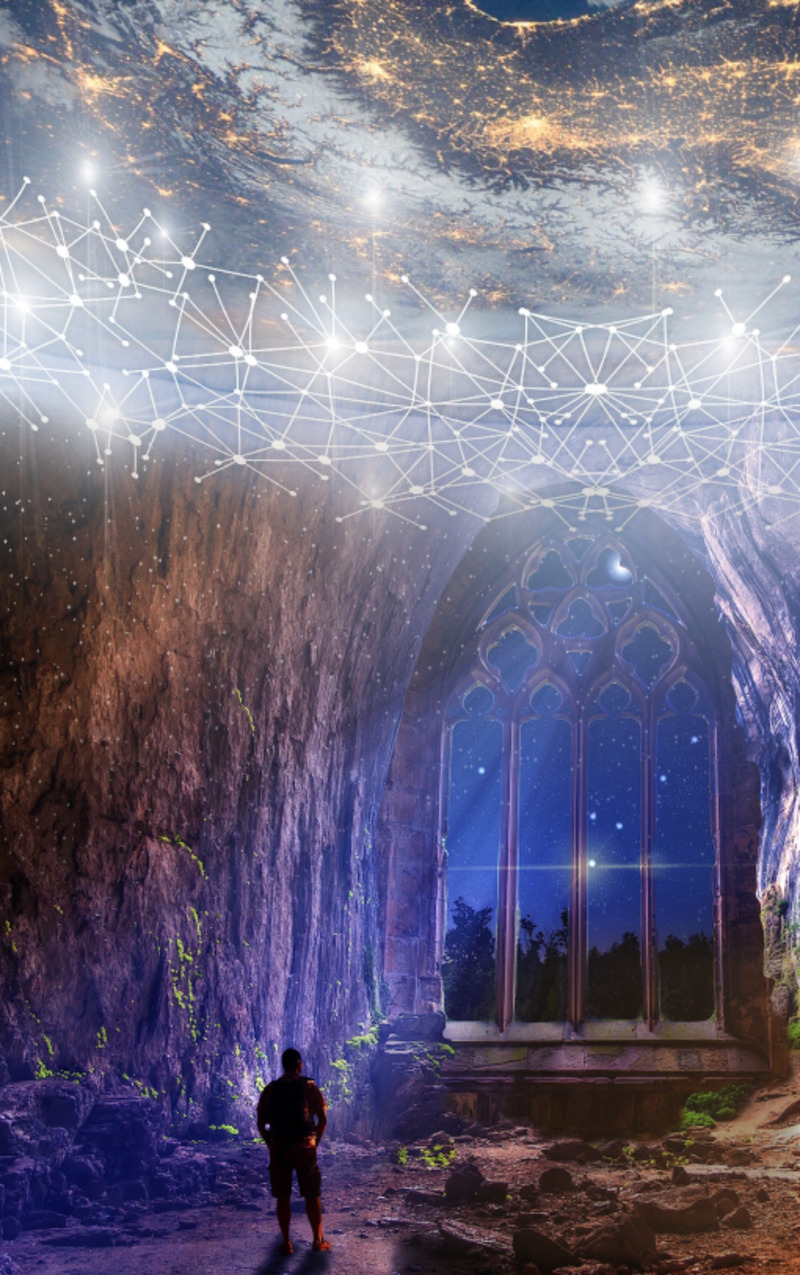
\includegraphics[width=1.01\paperwidth, height=1.01\paperheight,keepaspectratio]{./media/images/cover_splash}}
  }
  \BgThispage
  \tableofcontents*
  \noindent\LARGE{\textbf{Credits}}\medbreak
  \hrule
%  \noindent\rule{9cm}{0.4pt}%watch
  \smallskip
  \noindent\large{\color{red!50!black}{\textbf{Creator\,/\,Graphics\,/\,Author: D. Cooper
        Stevenson}}}\\
  \noindent\small{Cooper Stevenson dedicates himself to enabling fulfilling
    human experiences through the aesthetic use of technology. He lives with his
    wife, \emph{Deanna} and his two cats, \emph{Tiberius} and \emph{Chester}.}\\ \\
  \noindent\large{\color{red!50!black}{\textbf{Editor: Peter M.J. Gross}}}\\
  \noindent \small{Peter is an editor and online content
  specialist who has been entertained by interactive fiction since "\emph{Nord and
  Bert Couldn't Make Head or Tail of It}." He had to resort to a walkthrough in
  order to complete \emph{Trinity}, and he could never figure out \emph{A Mind Forever
    Voyaging}.}

\thispagestyle{empty} %clear header
\newpage
% First Article
\chapter*{}
\begin{textblock*}{70.9mm}(0mm,0mm)
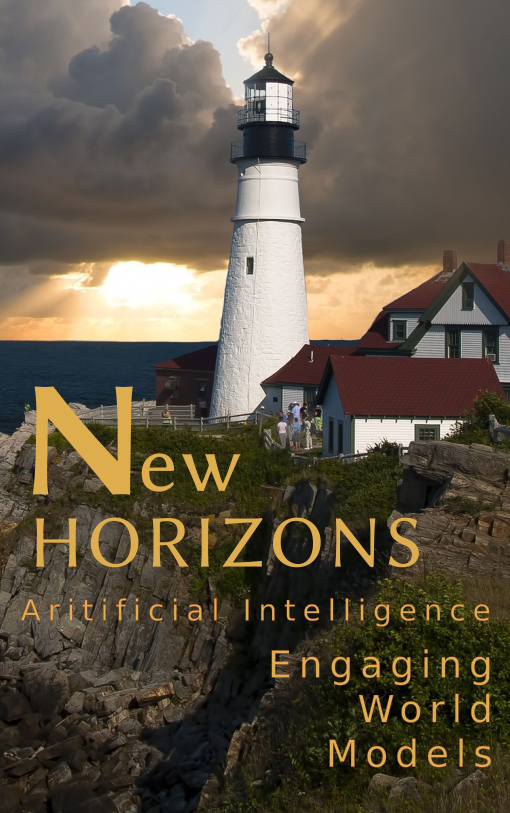
\includegraphics[width=\paperwidth]{./media/images/editorial_cover}
\end{textblock*}
\clearpage
\chapter{New Horizons\\ \small{Artificial Intelligence For Engaging World Models}}
\begin{figure*}[h]                                                           
 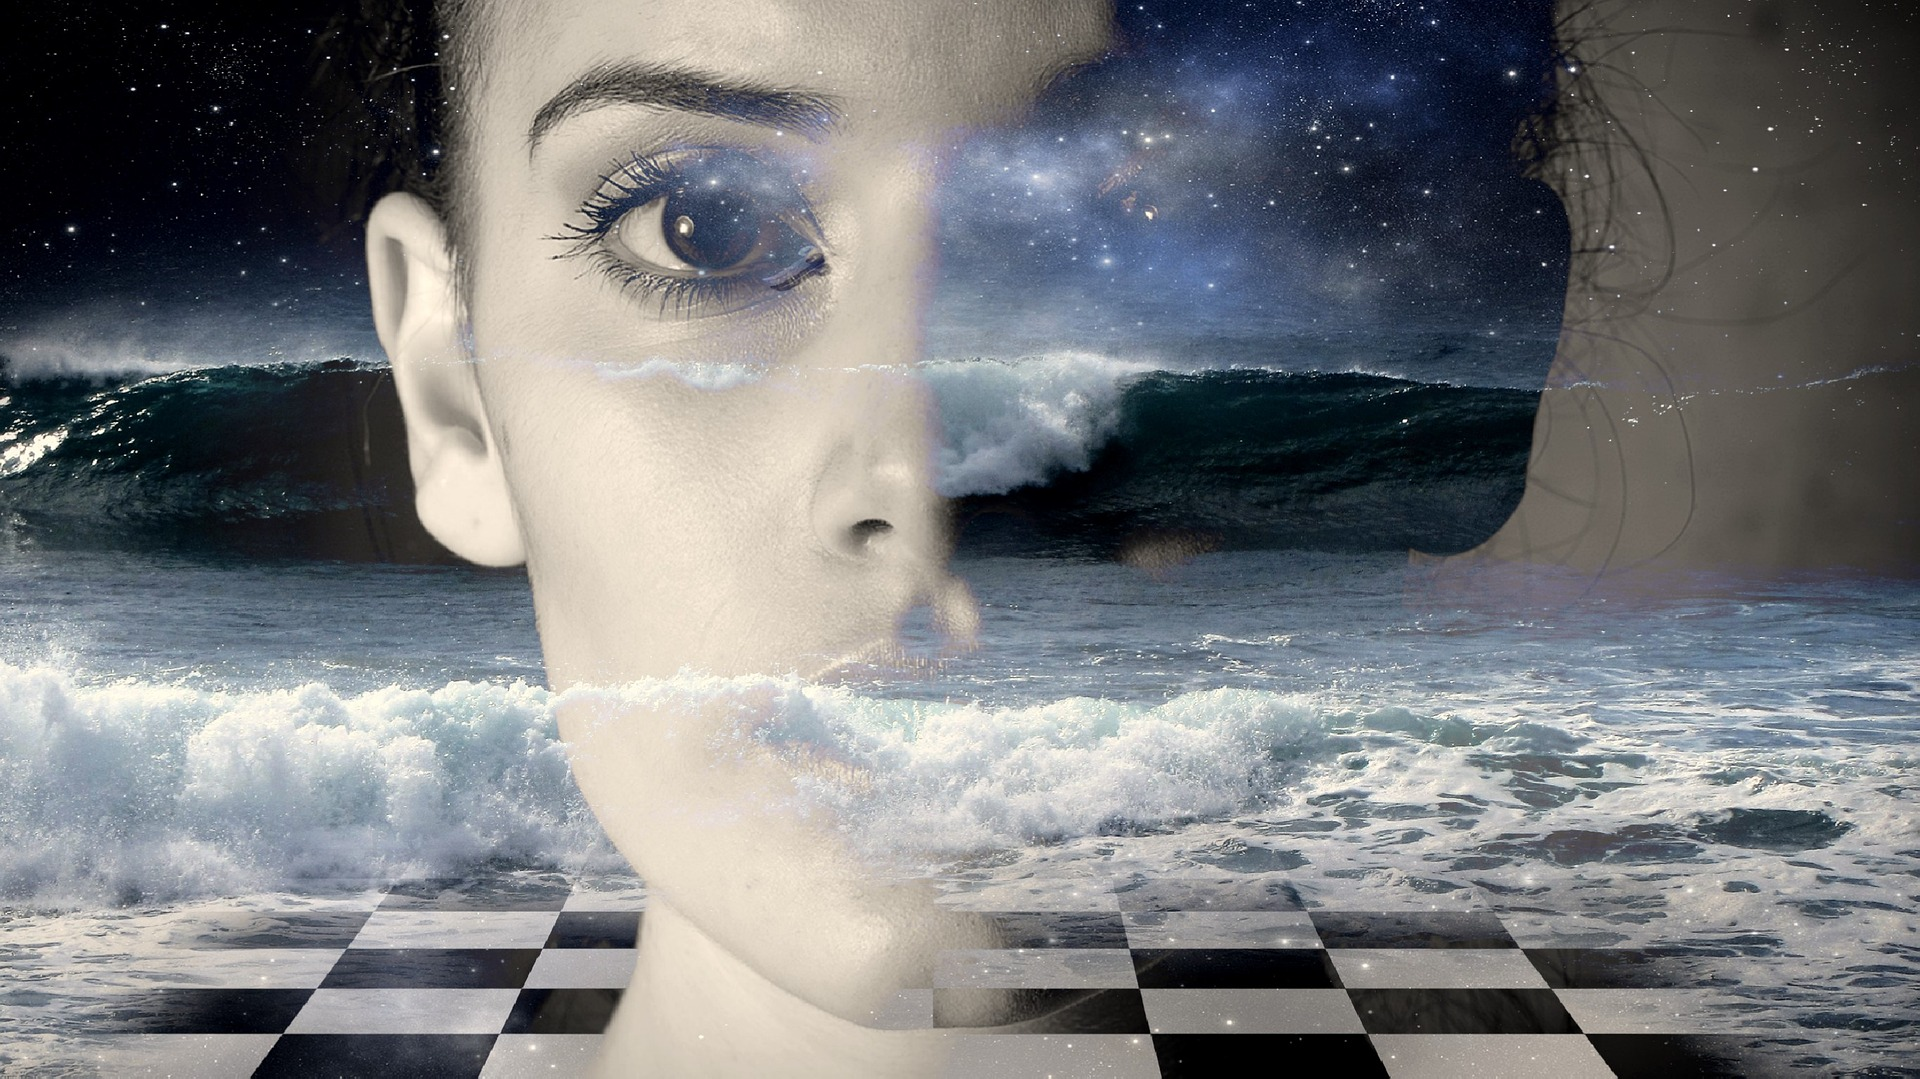
\includegraphics[width=\linewidth]{./media/images/chess.jpg}%
  \scriptsize{\textsc{\\we now have} effectively limitless capability to build
    dynamic, immersive world models.}
  \label{fig:editorial}%                                                 
\end{figure*}                                                                
\begin{quotation} 
\noindent\color{Sepia}{{\textit{\textbf{“Any sufficiently advanced technology is indistinguishable from magic.”
 }}}}\\[.5mm]
   \hfill\color{Sepia}{\small{\textendash Clarke's Law}}
\end{quotation} 
%\begin{abstract}
%\textbf{\emph{“In the beginning the Universe was created. This has made a lot of people very angry and been widely regarded as a bad move.”  \\ \\--- Douglas Adams}}
%\end{abstract}
\newpage
\marginnote{Editor's note: margin notes in red signify links pointing to sites of reference}[2em]
\lettrine[lines=3]{\color{BrickRed}I}{\enspace n} 1997 champion Gary Kasparov
lost to \textsc{ibm}'s ``Deep Blue'' supercomputer in a highly publicized
match.\reversemarginpar\marginnote{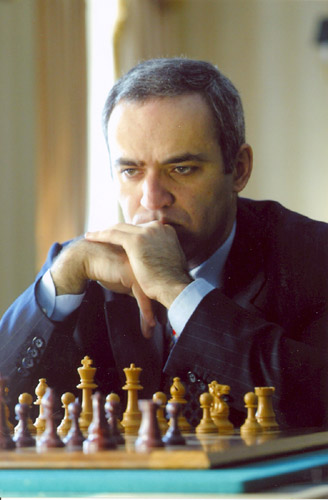
\includegraphics[width=\linewidth]{./media/images/gary}
  \href{https://www.youtube.com/watch?v=NJarxpYyoFI}{Gary Kasparov's match with
    ``Deep Blue'' was highly publicized and carried philisophical
    implications}}\label{img:kasparov}\pagenote[Page \pageref{img:kasparov}
World Champion Gary Kasparov]{Gary Kasparov image Copyright 2007, S.M.S.I., Inc.
  – Owen Williams, \href{http://www.kasparovagent.com/photo_gallery.php}{The
    Kasparov Agency},
  \href{https://commons.wikimedia.org/w/index.php?curid=4507357}{CC BY-SA 3.0}}
In 2011, \textsc{ibm}'s purpose\textendash built computer, named Watson and
developed to compete on the quiz show \textit{Jeopardy!}, prevailed over
legendary champions Brad Rutter and Ken Jennings to win first place and take the
\$1 million prize. In 2016, Google's
AlphaGo\normalmarginpar\marginnote{\href{https://en.wikipedia.org/wiki/AlphaGo}{Wikipedia:
    AlphaGo}}[-1em] computer program defeated the Go world champion, Lee Sedol, in a
five\textendash game professional match.
\marginnote{%\vspace{-6em}
  \href{https://www.youtube.com/watch?v=P18EdAKuC1U}{Watson prevailed over
    legendary champions Brad Rutter and Ken Jennings to win first place and the \$1 million prize}}\label{link:watson}In each case, the computer scientists is met with skepticism. In each case, the
dedicated technologists proved the skeptics wrong. At the crest of each new
achievement, philosophers asked the next logical questions thus restarting the cycle of discovery and progress.

By leveraging big data, artificial neural networks, and natural language
processing we can continue to explore new horizons.

%\marginnote{
%  {\href{https://en.wikipedia.org/wiki/Go_(game)}{Go}
%}

\section{socratic method of immersion}
What makes games so engaging is their way of pushing our human experience.
\marginnote{
  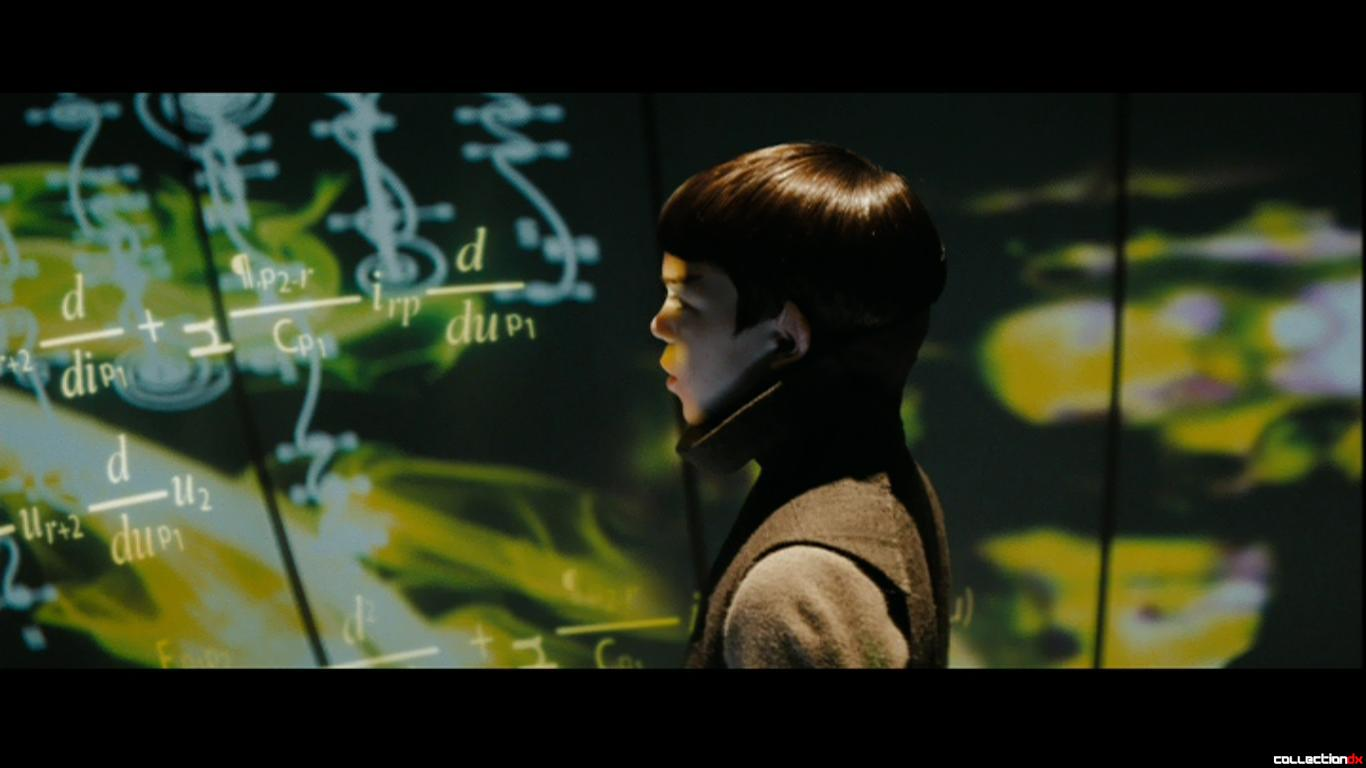
\includegraphics[width=\linewidth]{./media/images/spock}
  Spock's formative schooling in ``Star Trek'' depicts
      hyper\textendash interactive
    education
}\label{img:spock}
They patiently and quietly ask us to tackle tough problems on our own. They make
us search our knowledge and intuition. The quiet rewards for our struggles are
those moments in our lives when we feel like we accomplished the before
unattainable. Challenging, positive interactivity engages our souls. It makes us, ``better than yesterday.''

If engagement is a significant factor in 
quantifiably productive\marginnote{\href{https://www.sciencemag.org/news/2014/05/lectures-arent-just-boring-theyre-ineffective-too-study-finds}{Lectures aren't just boring they're ineffective too, study finds}}[2em] experiences then it stands to reason that a kind of Socratic ``give and take'' yields higher satisfaction and knowledge retention.
Interlocutors, like Kasparov or Sedol, query their environment. It replies with
meaningful responses. Similarly, the interactive question\textendash
and\textendash answer format of \textit{Jeopardy!} offers a distilled form of
mutual concession; it's mechanics lay bare the underpinnings of good Interactive
Fiction. When we ask intelligent questions of our world we expect fulfilling,
logical answers. When we get meaningful answers, we treasure that meaning like a prized possession.

\subsection{make it good}
\noindent Chris Crawford describes the value and nature of good
interactivity:
\begin{quote}
\marginnote{\href{https://youtu.be/3BPERIDSxKo?t=868}{Chris Crawford expresses
    the nauture and value of interactivity in an interview for ``Get Lamp''}}[2em]
The value of interactivity arises from the way the human mind responds to it.
The human mind is not a passive receptacle\textemdash it's an active agent. We don't learn
by sitting on our fat butts and listening or watching or hearing or passively
receiving information. We learn by reaching out to the world and messing around
with it with our fingers.
\end{quote}

\noindent Experience and research shows that high\textendash quality interactivity enhances the participants' satisfaction and
persistence with the content. \marginnote{\href{http://jolt.merlot.org/vol10no2/croxton_0614.pdf}{The Role of Interactivity in Student Satisfaction and Persistence in Online Learning}}
But the interactive environment must remain focused, substantively complete, and\textemdash most of
all\textemdash engaging. Understanding the power and fragility of interactive models
means understanding that the construction of solid frameworks is necessary from
the very start of our work.

Complete interactivity \textit{prima facie} implies that we need to
build a complete world model. By our ``completeness theory,'' the reader must be
able to rob a bank in a work of interactive
romance comedy, or else the system cannot provide plausible engagement.
Fortunately, experience  
suggests that total world modeling is not necessary for immersion. We find our
saving grace in the capability of our minds to suspend disbelief for the purpose
of enjoying the experience. 

In an interview for \textit{Get Lamp}, Crawford addresses\label{link:extent_model} the level of detail required for our world model
to provide credible stories:
\begin{quote}
\marginnote{\href{https://youtu.be/3BPERIDSxKo?t=1604}{Chris Crawford discusses
    the extent to which a complete world model is necessary in an interview for ``Get Lamp''}}[1em]A lot of people, I think, mis\textendash understand the nature of interactivity thinking that it requires giving the player absolute freedom. That's not at all what interactivity requires. It merely requires giving the player \textit{all relevant, useful freedom}.
\end{quote}
We've seen audiences enjoy and learn
from\marginnote{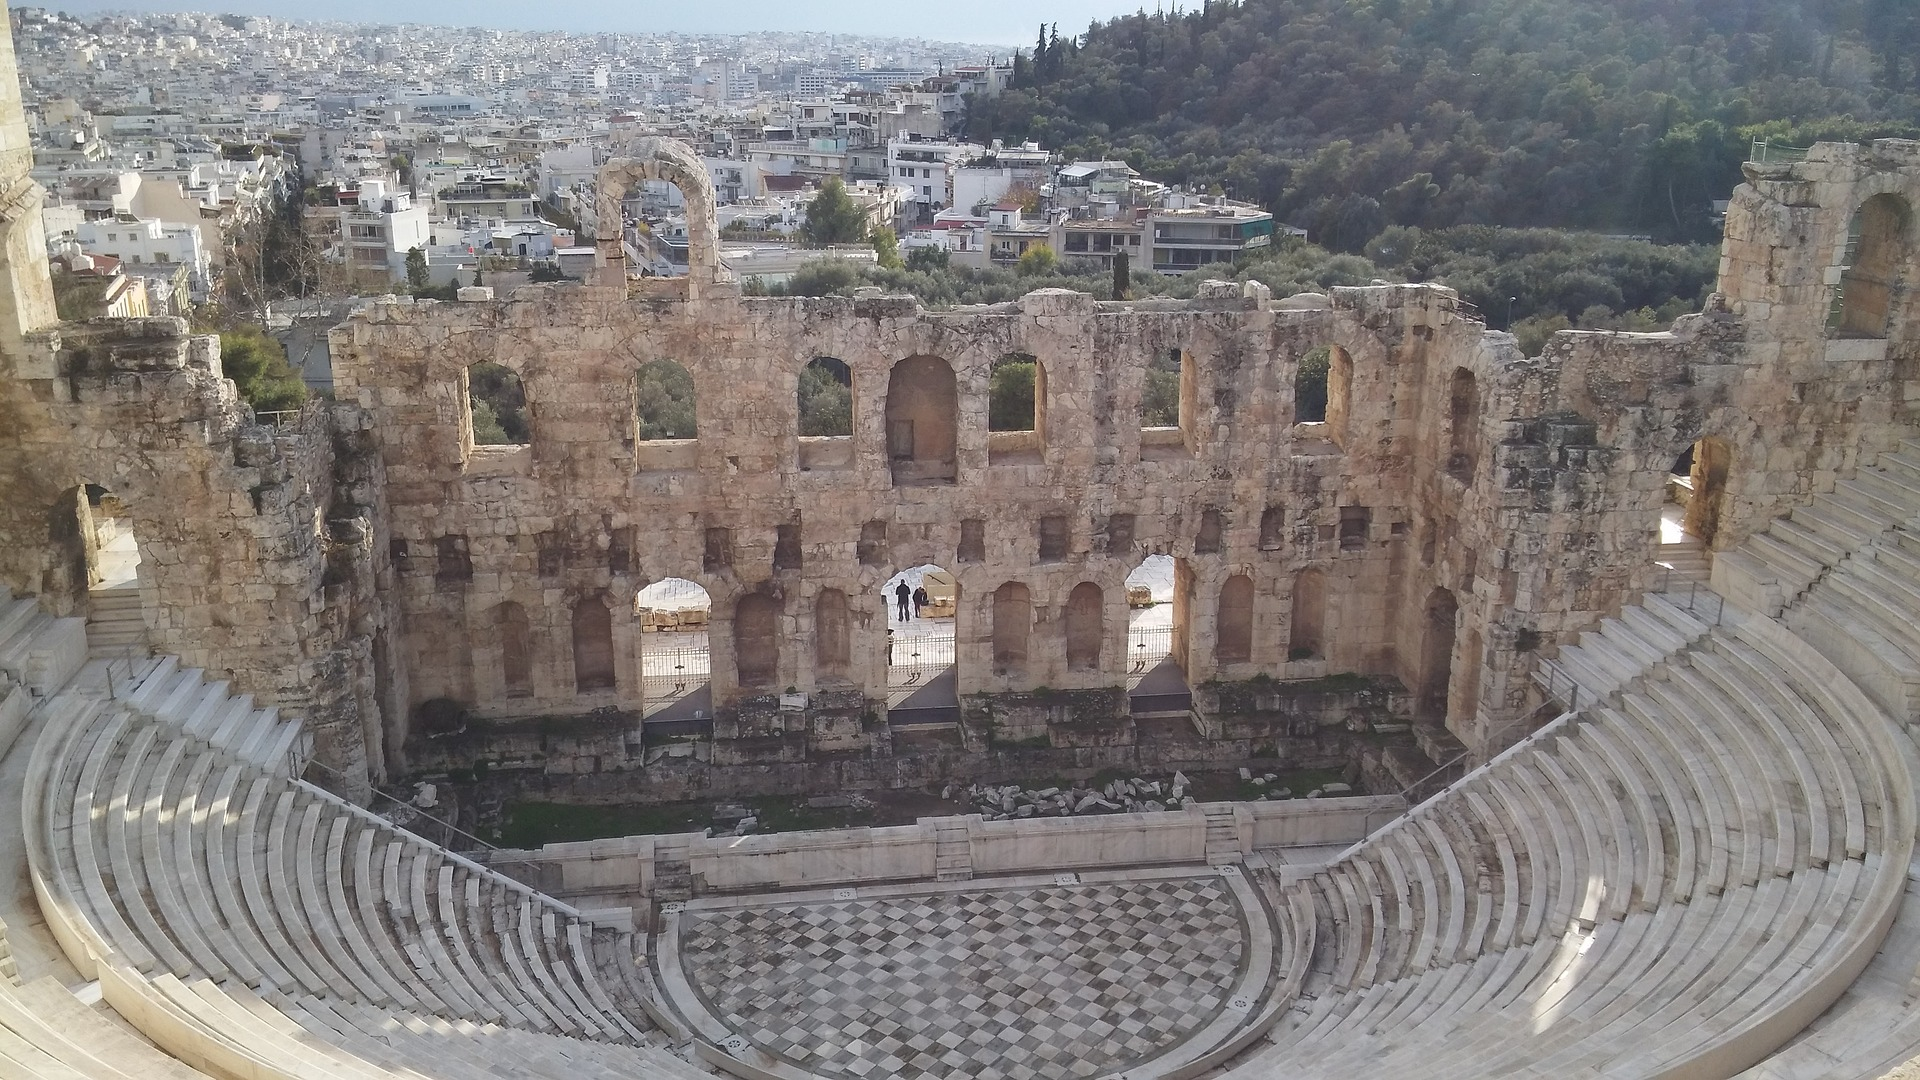
\includegraphics[width=\linewidth]{./media/images/greek_theatre}
  \tiny{\textit{Audiences consume themselves in stories while sitting on stone
      slabs through suspended disbelief}}} stories from as far back as the Greek
Tragedies, when great warriors and fair maidens entertained crowds that sat in
stadium style theaters on stone slabs. A story's efficacy doesn't come directly
from the physical setting of the audience. The theater sets the mood, while the
careful crafting of dialog, executed with superb timing, delivers the story's
impressions, which can be profound. The message speaks to us on primal levels
that
\marginnote{\href{https://greatergood.berkeley.edu/article/item/how_stories_change_brain}{Paul
    J. Zak, How Stories Change the Brain}} can be measured. Beyond the science,
writers deliver experiences by relying less on settings and more on \textit{story}.
\subsection{the struggle eternal}
Writing complete Interactive
  Fiction worlds by hand is a long, arduous process. There's no way around it. 
Aaron Reed, in an interview for \textit{Get Lamp} notes,
\begin{quote}
\marginnote{\href{https://youtu.be/LRhbcDzbGSU?t=2575}{Aaron Reed notes the
    complexities of creating a complete world model in \textsc{if}}}[2em]
As a player of Interactive Fiction, it's very easy to not appreciate the work
that went into it. You just come across one error message or one response that
the designer didn't think of and you think, ``Oh, well, forget this game.''
After you've actually gone through and had to think of all those things and code
them and write them yourself, your perspective really changes.
\end{quote}

\noindent Complete world models, on the other hand, where the Interlocutor feels confident that their
interactions will be met with meaningful responses is known to be the most
important factor in their enjoyment of Interactive Fiction. Emily Short writes
in her article, ``The Prose medium and \textsc{if}:''
    \begin{quote}
    \marginnote{\href{https://emshort.blog/how-to-play/writing-if/my-articles/the-prose-medium-and-if/}{Emily
        Short considers the reltionship between prose and parser function in, ``The Prose medium and \textsc{if}''}}[2em]
    By contrast, negative points made about \textsc{if} in the wider world (and here I draw
    from threads on \textsc{slashdot} about the yearly comp, and discussions on various
    gaming boards) often focus on the parser, not the writing, as the critical
    weakness of \textsc{if}. It is the refusal to recognize nouns mentioned in the text, the
    insistence on very particular player behavior, the guess-the-verb nonsense,
    that turns off the most people, as I observe it.
    \end{quote}
So it is that precisely what the reader finds most important to a good work of
\textsc{if} turns out to be the most burdensome for the implementer to write.
The implementer's task isn't limited simply by sheer mass of the world's
components; his undertaking is compounded in difficulty by the fact that he must
think of everything a reasonable reader will try to do in the world for any
given situation. The player's complete agency and the implementer's difficulty
furnishing his world model mix like oil and water.

\subsection{critical non\textendash acclaim}
Some argue the readers expectation of agency and the implementors burden to
achieve the goal will never resolve. They will say that there is no way an
implementor will come even close to a satisfactory world model without resorting
to trite gimmiks. Proponents of this argument point to efforts in the past, most
of which have fallen short. They will pine eloquent about the absolute
complexities of the task's implied workload and call upon the implmenter as
running a fool's errand.

To the critics I respond as Theodore ``Teddy'' Roosevelt did,
\begin{quote}
It is not the critic who counts; not the man who points out how the strong man stumbles, or where the doer of deeds could have done them better. The credit belongs to the man who is actually in the arena, whose face is marred by dust and sweat and blood; who strives valiantly; who errs, who comes short again and again, because there is no effort without error and shortcoming; but who does actually strive to do the deeds; who knows great enthusiasms, the great devotions; who spends himself in a worthy cause; who at the best knows in the end the triumph of high achievement, and who at the worst, if he fails, at least fails while daring greatly, so that his place shall never be with those cold and timid souls who neither know victory nor defeat.
\end{quote}
I argue that, given today's \textsc{if} authoring technology to works of the
past is a little like comparing the Nicéphore Niépce's first fixed image with a
camera to today's moving experiences found in modern film.

We have virtually no limit on the size and scope of our work and we can use all
available mediums in the world model through scripting hooks available with both
\textsc{tads3} and \textsc{inform 7}. I submit boldly that it ought even
be possible using projectors to let players roam around in a physical building
or geodesic dome where the rooms, using projectors, change as the story does.

\includepdf[scale=1.01]{media/images/dating_ad.pdf}

\subsection{critical constructs}
The question of creating rich, virtual experiences quickly escalates into
varying narrative techniques and structures, fluid linguistics, and other
aspects. I will
happily leave these discussions to the scholars as we focus on creating a
foundation that they may all build on. Our goal is to build an efficient and flexible framework whose capabilities enable all comers. 

The solution, whatever it may be, should answer this core question: ``How do we build
an engaging world whose dynamics deliver enriching engagement for the
audience?'' We assume no bounds and take only the requirement for verifiable
results to achieve our goal. If our work passes a literary Turing
Test\marginnote{\href{https://en.wikipedia.org/wiki/Turing_test}{Wikipedia:
    Touring Test}}, we are successful. Hopefully (and probably), we've created a
framework for others to follow and develop further. Our story's positive effect on the audience is our mission.

To date I know of no substitute for inspired creativity. There exists no
system\textemdash quantum or otherwise\textemdash that serves even as a shallow replacement
for inspiration. Our minds possess sophisticated neural methods for spotting
contrivance at a glance. We're embroiled in
an\marginnote{\href{http://theconversation.com/the-evolution-of-lying-14254}{Rob
    Brooks, The Evolution of Lying}} arms race between lying and honesty
detection that continues to this day. And so far the longevity of inspired works
shows a direct correlation with honesty; Plato's ``The Republic'' survives to this day, while last month's ``Enquirer'' headlines do not.

That is the first plank of our system's foundation: raw inspiration
space for the writers expressing their brutal honesty. There's no ``man behind the
curtain'' in our model. Just as Greek theaters made no claim to be
a of being Greco-Punic battlefields, we make no claims that our emulated world
is a complete manifestation of the real environment. ``However,'' we say, ``if you let
us, we will take you on a journey of laughter, sadness, or possibly both.
Perhaps we will make you think in ways you have never thought before. Above all, we will make you \textit{feel}.''


\subsection{nuts and bolts}

This issue of \textit{Discoverer's Digest} provides
step{\textendash}by{\textendash}step instructions to build topic modeling and natural language
processing systems that can greatly reduce the effort required to build your world and
narrative models. Building an authentic world requires an enormous amount of
writing; these techniques can assist greatly by generating ideas and taking care
of the mundane. The author may focus on \textit{story} rather than clerical
tasks and associations.

Both techniques draw (or can draw) their results from the entire collection of Wikipedia articles
(all 5.7 \emph{million} of them, in English alone). It's as if the entire collection human thought was at
your disposal to build your work of
Interactive Fiction. The result is a systematized method for creating complete,
relevant world models.

Topic modeling is a systematic way to flesh out 
areas that are related to a work's central themes\textemdash the broad areas that an
Interactive Fiction audience is likely to
explore. Topic modeling also helps generate completely new areas of reference
we often hadn't thought of.

It provides a ready\textendash made system that suggests
the most relevant topics for a query. Those topics
can be re\textendash entered into the system to provide greater depth and
generate additional detail with more
relevant topics, and so on.

The issue also discusses natural language processing, where we select a subject or
word phrase to see how it is used in context with surrounding text. It provides 
brief phrases that span multiple contexts for works of Interactive Fiction.

Both articles are somewhat technical. However, the step\textendash by\textendash
step instructions should make it easy to replicate their results; each step is
explained along the way. These articles use the \textsc{linux} operating
system but their techniques may be adapted for other operating systems.

% * We don't have issues of memory limits anymore
% * [[https://github.com/danielricks/scholar][Using linear algebra, we were able to pull affordances (relevant verbs) for nouns out of word2vec, with varying success on other parts of speech. This interface provides methods that perform those operations.]]
% ** So, with this, we feed the nouns in and get a list of relevant verbs, e.g.
% DOG: 'pet dog, kick dog, call dog, etc.'

% Look, I'm not suggesting the world will make the story--only polished work and
% rewrites will do that. But should we enslave ourselves to have to write the
% world from scratch?

% Of course, this isn't 
% This is what I hope to make a small dent toward achieving.

All in all, this issue provides foundational frameworks to build the
scope and context of your authorship quickly, assisting with contextual phrasing for each
geographic or narrative node in your story. Running your topics and phrases
through these systems will provide you with quick ``stubs'' to support 
your work. Its suggestions will provide moments where you think, ``ah, it's true that \textit{x} is related to
\textit{y}, I didn't think of that.''

I hope you enjoy this magazine. \emph{Discoverer's Digest } seeks to cover all manner of
topics related to Interactive Fiction, ranging from parser experiences to
choice\textemdash games, along with experiments in the medium (including General Artificial Intelligence) that we've not yet seen.

And please submit your news, story ideas, and comments by sending a personal email to \href{mailto:cooper@discdigest.xyz}{cooper@discdigest.xyz}. \\ \\

\noindent Happy Writing! \\ \\

\noindent \href{mailto:cooper@discdigest.xyz}{\textsc{D. Cooper Stevenson}}


\chapter*{}
 \begin{textblock*}{70.9mm}(0mm,0mm)
   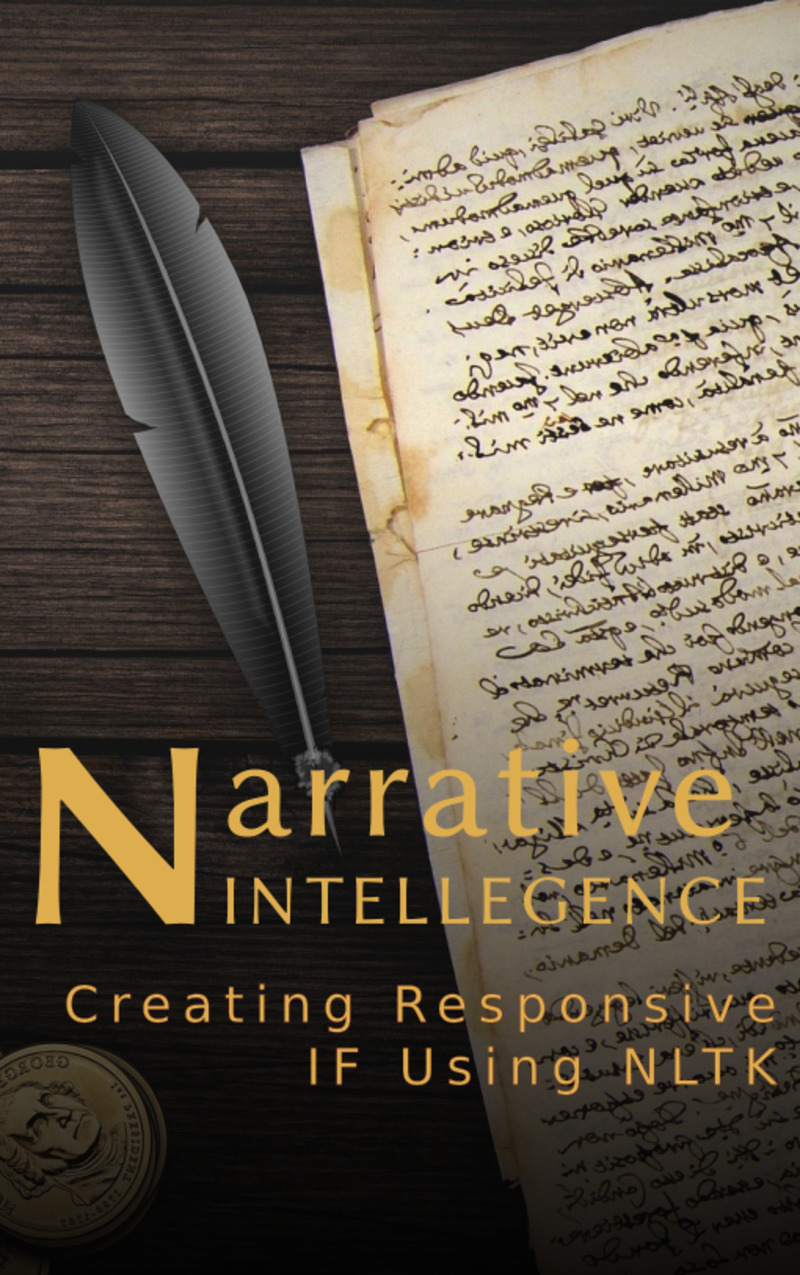
\includegraphics[width=\paperwidth]{./media/images/nltk_cover}
 \end{textblock*}
 \chapter{Narrative Intelligence\\ \small{Creating Responsive IF Using NLTK}}
 \begin{figure*}[h]                                                           
 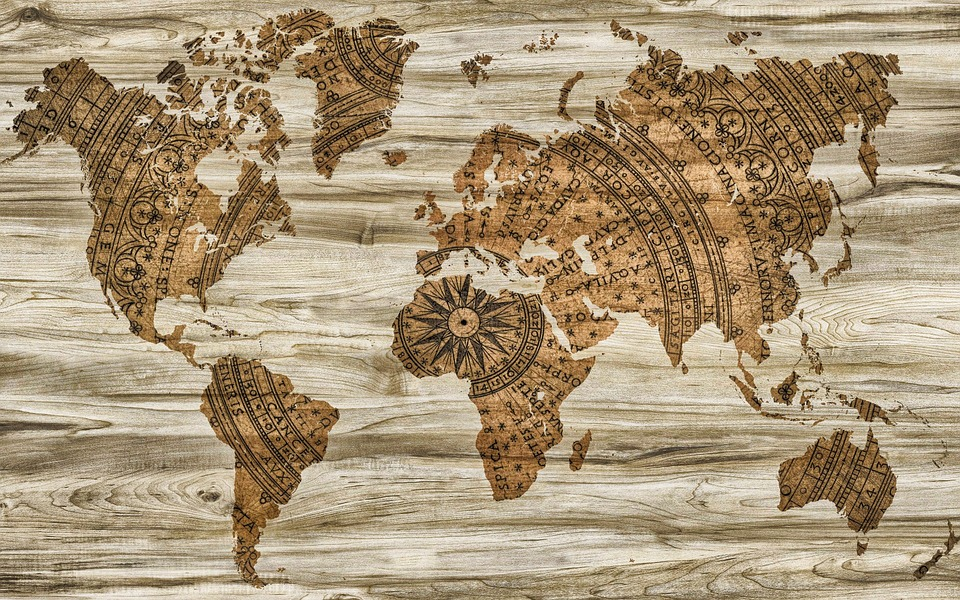
\includegraphics[width=\linewidth]{./media/images/world_map}%
  \scriptsize{\textsc{\\removing the burden} to implement every detail goes a
    long way toward creating polished \textsc{if} environments}
  \label{fig:editorial}%                                                 
\end{figure*}                                                                

\begin{quotation} 
  \noindent\color{Sepia}{\textit{\textbf{“If you put yourself in a position where you have to stretch outside your comfort zone, then you are forced to expand your consciousness.”}}}\\[.5mm]
   \hfill\color{Sepia}{\small{\textendash Les Brown}}
\end{quotation} 
\newpage
\lettrine[lines=3]{\color{BrickRed}N}{\enspace atural Language Processing}
[\textsc{nltk}] may hold the key to breakthrough levels of engagement in
\textsc{if}. It's power lies in it's ability to query
millions of lines of text, retrieve quantified answers in the source
material, and bring relationships between entities to light. The context
suggestions translate into actionable intelligence
for the author and greater submersion for the reader. \textsc{nltk}'s
ability to retrieve massive numbers of contexts and relationships in seconds
make it's techniques powerful instruments for building immersive world models.

\marginnote{\href{http://sapir.psych.wisc.edu/programming_for_psychologists/cheat_sheets/Text-Analysis-with-NLTK-Cheatsheet.pdf}{Text analysis with \textsc{nltk} cheatsheet}}[2em]
\textsc{nltk} is not only fast it's architecture lends itself to automation.
Once the author selects the topics to be covered\textemdash likely using topic modeling
as described beginning on page \pageref{sec:topic}\textemdash an article summarizer is
used to pull out each topics' salient features.
These results are fed into \textsc{nltk} for context, parts\textendash
of\textendash speech, and related associations specific to each result. Natural
language processing with \textsc{nltk}'s modular architecture provides volumes of
relevant results that can be molded to suit your workflow.

%TODO: Link to nltk cheatsheet

Responses for all kinds of player queries can be 
built efficiently using \textsc{nltk}'s features:
\begin{itemize}
  \setlength\itemsep{0em}
  \item{Varying, sometimes wide\textendash ranging contexts for a particular topic or object}
  \item{Brings forward parser responses you may not have considered}
  \item{Tags objects mentioned in the main prose to avoid ``I don't see any x
      here'' here messages}
\end{itemize}
%I'll outline examples of each with examples and provide a brief tutorial for
%configuring your system to run \textsc{nltk}.
\section{a time and a place}
\marginnote{Corpos: nothing more than a large body of text, sometimes referred to as, ``a big bag of words''}[1em]
Suppose we're writing a character modeled after Captain Ahab in the seminal
classic, ``Moby Dick.'' After loading the Moby Dick corpus, included with
\textsc{nltk}, we query the system for where Captain Ahab appears in context:
\pagebreak

\marginnote{These results appear as broken English because the corpus is processed to remove ``stop words,'' i.e. ``the, a, that,'' etc. Run your queries against raw corpus text if you want results in complete sentences.}[5em]
\begin{lstlisting}
  >>> text1.concordance('ahab')

, eh ? Have ye clapped eye on Captain Ahab ?" " Who is Captain Ahab , sir ?" " A
e on Captain Ahab ?" " Who is Captain Ahab , sir ?" " Aye , aye , I thought so .
 " Aye , aye , I thought so . Captain Ahab is the Captain of this ship ." " I am
ast backing out . Clap eye on Captain Ahab , young man , and thou wilt find that
ptain Peleg , inquiring where Captain Ahab was to be found . " And what dost tho
 " And what dost thou want of Captain Ahab ? It ' s all right enough ; thou art
l thee . He ' s a queer man , Captain Ahab -- so some think -- but a good one .
 , ungodly , god - like man , Captain Ahab ; doesn ' t speak much ; but , when h
ll listen . Mark ye , be forewarned ; Ahab ' s above the common ; Ahab ' s been
ewarned ; Ahab ' s above the common ; Ahab ' s been in colleges , as well as ' m
\end{lstlisting}

From the results we can see that he is a Captain of a ship, educated, is ``above
the common,'' and keeps his thoughts close to his chest overall. Immediately we
find that we can ask Ahab about topics like his ship, his education, and his mission (if he'll
tell us). If we observe closely, we find clues to his personality. This phrase
is intriguing:
\begin{lstlisting}
  , ungodly , god - like man , Captain Ahab ; doesn ' t speak much ; but , when h
\end{lstlisting}

Let's learn more

\begin{lstlisting}
  >>> text1.concordance('speak')
 ' t speak much ; but , when he does speak , then you may well listen . Mark ye
\end{lstlisting}
According to at least one character in the book (who knows Capatain Ahab well as
other queries attest), Captain Ahab is a quiet man but should be listened to
when he does speak.

Notice through shaping our character so far we've not had to ``think'' of
anything\textemdash the system digs through the corpus and provides us with a profile for
our subject of interest.


\includepdf[scale=1.01]{media/images/sailor_ad.pdf}
\section{saving mimesis}
Alright, so we write our character based on Captain Ahab. Let's call him
``Captain Moby'' (sacrilege, I know):
\begin{quote}
Captain Moby leans slightly forward as he scans the horizon from the fore deck
of his ship, ``\textit{Pequod.}'' 
\end{quote}
  An interaction like this would break nimesis:
  \begin{lstlisting}
    > examine Pequod
    I don't see any Pequod here.
  \end{lstlisting}
\marginnote{\href{http://pdf.textfiles.com/books/iftheorybook.pdf}{Roger Sorolla, ``Crimes Against Mimesis'' {\textsc{(pdf)}}}}[1em]
\textsc{nltk} can help with this by taking our prose through a parts\textendash of\textendash speech parser:

\begin{lstlisting}%[basicstyle=\tiny]
>>> mytext = nltk.word_tokenize("Captain Moby leans slightly forward as he scans the horizon from the fore deck of his ship, Pequod.")
>>> nltk.pos_tag(mytext)
[('Captain', 'NNP'), ('Moby', 'NNP'), ('leans', 'VBZ'), ('slightly', 'RB'), ('forward', 'RB'), ('as', 'IN'), ('he', 'PRP'), ('scans', 'VBZ'), ('the', 'DT'), ('horizon', 'NN'), ('from', 'IN'), ('the', 'DT'), ('fore', 'NN'), ('deck', 'NN'), ('of', 'IN'), ('his', 'PRP\$'), ('ship', 'NN'), (',', ','), ('Pequod', 'NNP'), ('.', '.')]
\end{lstlisting}
Here we're looking for Proper nouns (NNP), and nouns (NN). In seconds we're
provided the following actionable items:
\begin{multicols}{2}
\begin{itemize}\setlength\itemsep{0em}
  \item Captain
  \item Moby
  \item horizon
  \item fore
  \item deck
  \item ship
  \item Pequod
\end{itemize}
\end{multicols}
\marginnote{\href{https://www.smithsonianmag.com/history/the-true-life-horror-that-inspired-moby-dick-17576/}{Fun fact: Moby Dick is based on a true story about Captain George Pollard Jr.}}[1em]
\noindent Does the system respond reasonably to, \emph{``examine Pequod''} or
\emph{``examine fore''}? Using the parts\textendash of\textendash speech tager,
yes, we're able to cover all relevant areas in each passage's prose. Your work's
manuscript can be used as input to produce a list of objects for implementation,
perhaps even, creating object templates that have ``TODO'' placed in them saving you the trouble of having to
write it yourself.

If we run an \textsc{nltk} 'similar' query like we did above on the word,
\emph{pequod}, by the way, we get this:
\pagebreak
\begin{lstlisting}
>>> text1.concordance('pequod',lines=10)
Displaying 10 of 25 matches:
...
rare old craft as this same rare old Pequod . She was a ship of the old school ,
to me and Captain Bildad to see the Pequod fitted out for the voyage , and supp
aling I must , and I would ; and the Pequod was as good a ship as any -- I thoug
...
\end{lstlisting}
We now see that the \emph{Pequod} is a commissioned ship of the stoutest breed
of ``old schol'' nautical design and construction.

Notice that the character in our story is modeled from a single
corpus. You can also craft your character with references from several bodies of
work. Other characters can be modeled after completely
separate works; the antagonist in your story could be modeled after
Shakespeare's \textit{Othello}. There are virtually endless ways of customizing
your source material in your work of \textsc{if}.
\section{installation}
Fortunately, installing \textsc{nltk} is fairly straightforward; you need only
python, \textsc{nltk}, and \textsc{nltk-data} installed to use the examples
described here.

\subsection{installing python}
Linux systems, almost without exception \textit{will} have \textsc{python} and \textsc{nltk}
packages available as standard. Here are the commands to install \textsc{python}
for various distributions:\\[1em]
For Debian/Ubuntu:
\begin{lstlisting}
  sudo apt-get install python3 python3-pip
\end{lstlisting}
For Arch Linux:
\begin{lstlisting}
  sudo pacman -S python python-pip
\end{lstlisting}
\marginnote{\href{https://www.python.org/downloads/windows/}{Python for windows download page}}[0.5em]
Windows systems may download \textsc{python} from the link found in the margin notes on this page. I
recommend using 
\textsc{powershell} when working with \textsc{python} and
\textsc{nltk}.Alternatively, in environments where Windows must be used as the
base operating system, it’s best to run these applications inside a virtual
machine running linux or bsd for industrial grade text processing.
\marginnote{\href{https://docs.python.org/3/using/windows.html}{Python documentation, ``Python on Windows''}}[-2em]
\subsection{installing nltk}
It's almost always better to stay inside the distribution's method for
installing \textsc{python} applications without resorting to \textsc{pip} or
other \textsc{python}
installation systems. Conflicts will occur if a dependency is
installed with \textsc{pip} when the package manager finds that the dependency is already installed. For \textsc{nltk} the installation looks like this:\\[1em]
For Debian/Ubuntu:
\begin{lstlisting}
  sudo apt-get install python-nltk 
\end{lstlisting}
For Arch Linux:
\begin{lstlisting}
  sudo pacman -S python-nltk nltk-data
\end{lstlisting}

For all operating systems I recommend downloading all the available
\textsc{nltk} packages; you will save a lot of time later not having to
worry about whether or not a required package is installed for a given
\textsc{nltk} operation:
\begin{lstlisting}
>>> import nltk
>>> nltk.download()
\end{lstlisting}
\begin{figure*}[ht]
\centering
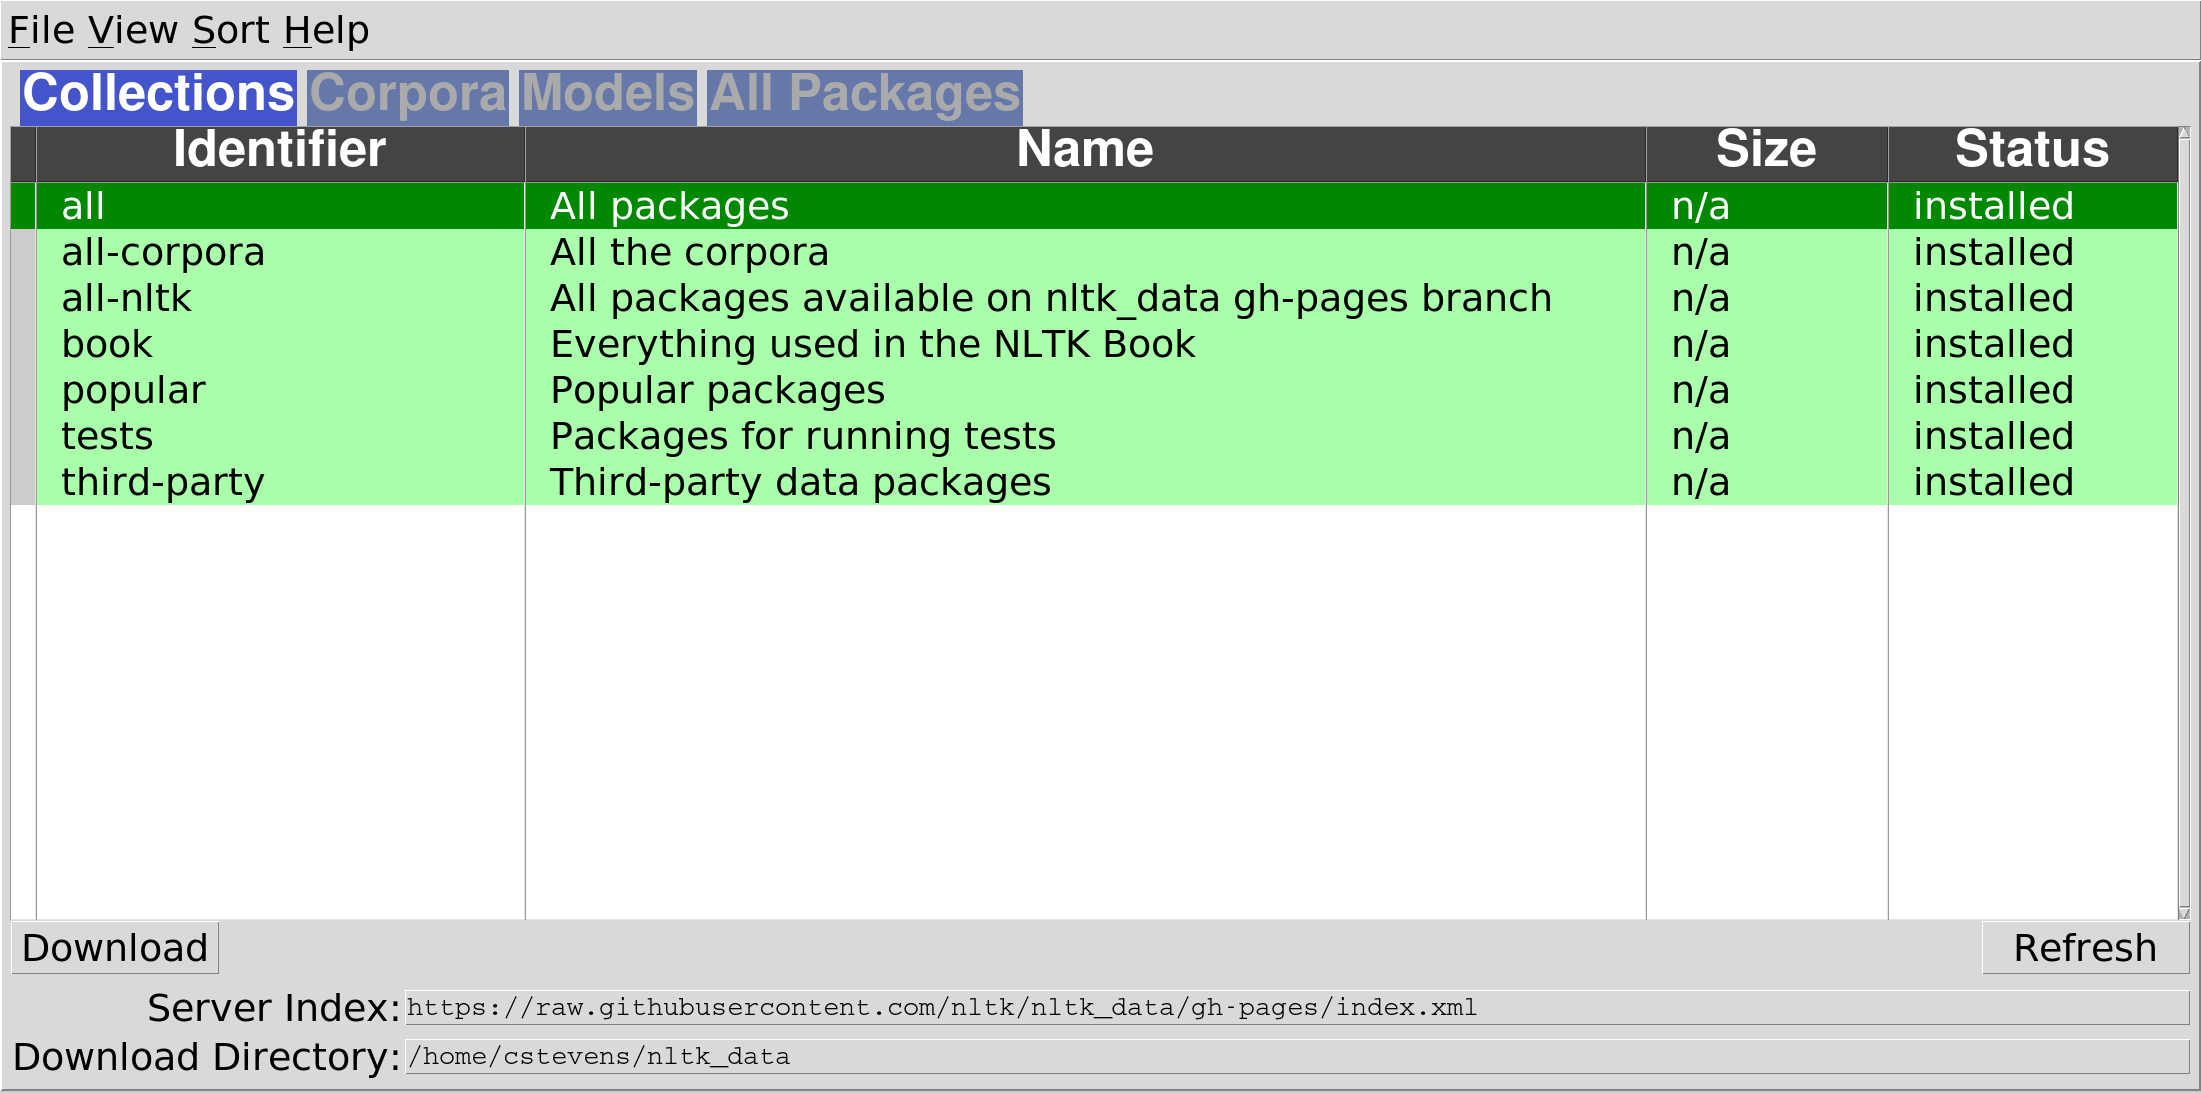
\includegraphics[width=\textwidth]{media/images/nltk_data.png}
  \caption{\textsc{nltk dialog for} installing \textsc{nltk} data packages}
\end{figure*}
\section{running queries}
Once \textsc{python} and \textsc{nltk} are installed you may run queries like
those outlined at the beginning of the article.

First, enter the \textsc{python} environment:
\begin{lstlisting}
  \$ python
\end{lstlisting}
\begin{figure*}[ht]
\centering
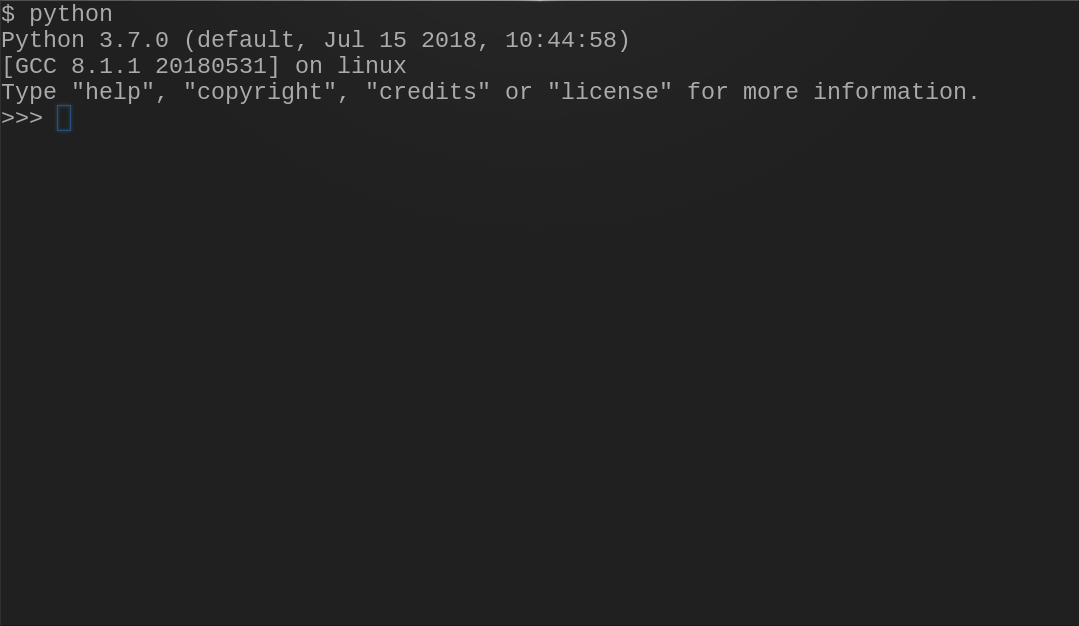
\includegraphics[width=\textwidth]{media/images/python_prompt.png}
  \caption{\textsc{entering the} python environment}
\end{figure*}
Next, we'll load the \textsc{nltk} library and default text corpus included in \textsc{nltk}:
\begin{lstlisting}
  >>> from nltk.book import *
\end{lstlisting}
\begin{figure*}[ht]
\centering
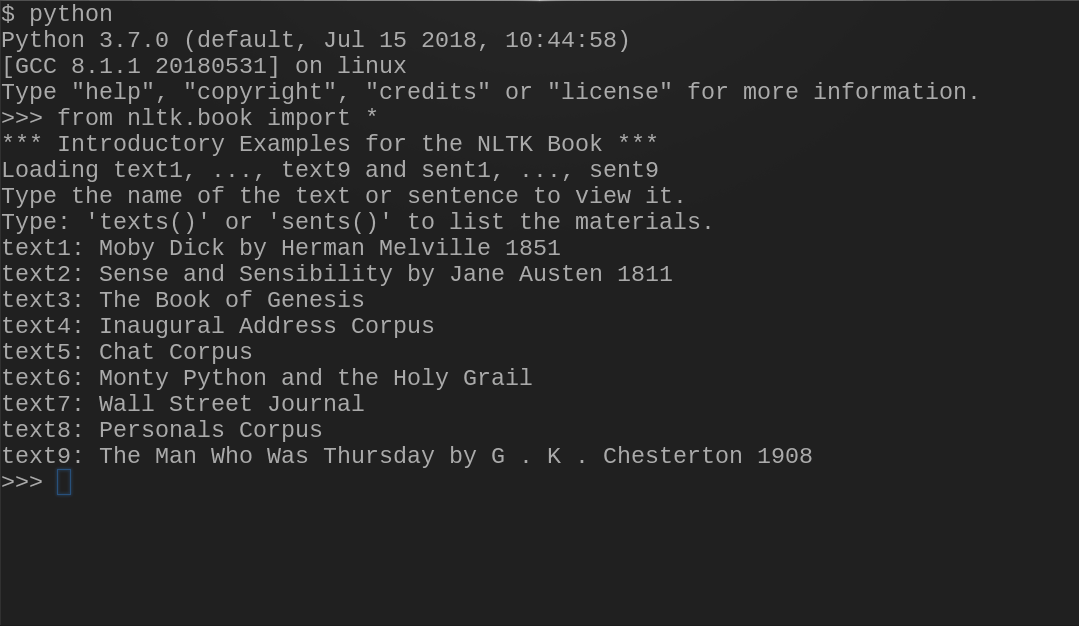
\includegraphics[width=\textwidth]{media/images/nltk_book.png}
  \caption{\textsc{nltk and test data} loaded and ready to receive natural
    language processing requests}
\end{figure*}
Notice the \texttt{\small{text1:, text2:,}} etc. designations. We use these designations
to specify a corpus we'd like to use when querying the data:
\begin{lstlisting}[language=Python]
  >>> text1.concordance('ahab',lines=2)
\end{lstlisting}
\begin{figure*}[ht]
\centering
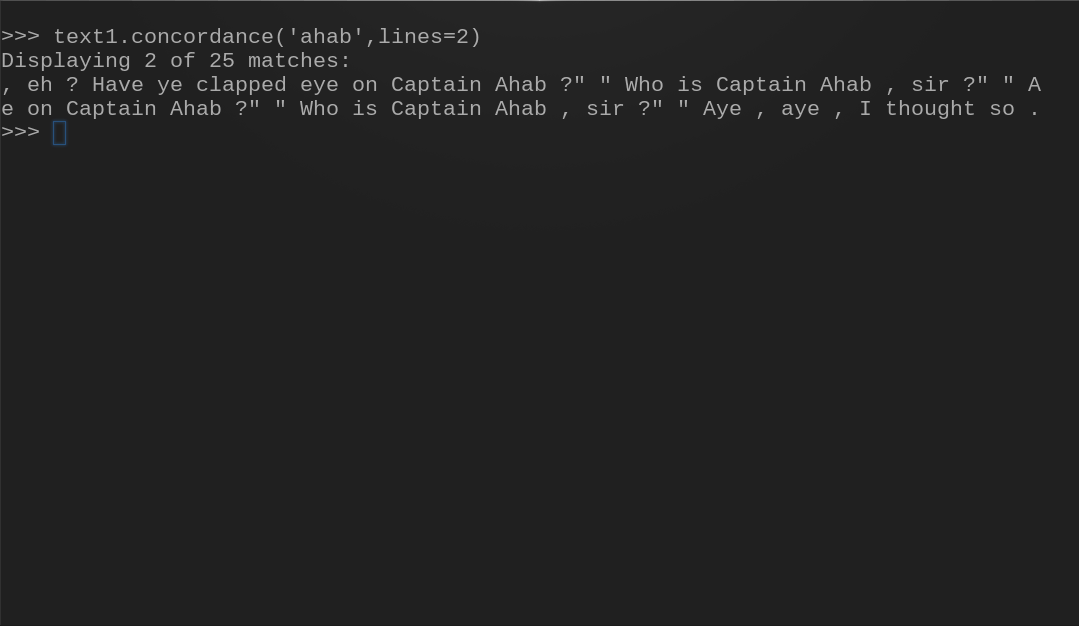
\includegraphics[width=\textwidth]{media/images/python_concord.png}
  \caption{\textsc{querying the 'moby dick'} corpus with the word, 'ahab'}
\end{figure*}
\textsc{nltk} lets you query different types of source data for
different purposes. Perhaps one character in your narrative is a romantic; you
could get insight into his personality by querying a work like
Shakespeare's \textit{Hamlet}. Alternatively, a powerful general may
be best served by \textit{Secret of the Night} by Gaston Leroux. Several works
of the same type may also be combined into a single
corpora for an even broader scope of natural language processing responses.
\section{divide and conquer}
These tools, coupled with custom corpus, make it possible to write scripts to search, tag and template hundreds or thousands of
connections automatically for author review and final implementation.
Automating \textsc{nltk} also works when dividing the work into teams. 

For example, after the creators provide the technical staff with the body of
works they wish to reference in their story a natural language processing based
workflow may look something like this:

\begin{itemize}\setlength\itemsep{0em}
\item Technologists code \& test the automation routines to place \textsc{nltk}
  query results into graphs (e.g. \textsc{graphiz}) 
\item Authors review the graphs containing the results and entity relationships for quality
\item Technologists run automation routines to convert the modified graphs into \textsc{tads3} templates
\item Artists \& authors review the output and modify it
\item Beta testers test, and transcripts are re\textendash entered into the
  natural processing loop as required
\end{itemize}
Of course, all the work, of course, is channeled through a revision system so
everyone receives timely updates.

\chapter*{}
 \begin{textblock*}{70.9mm}(0mm,0mm)
   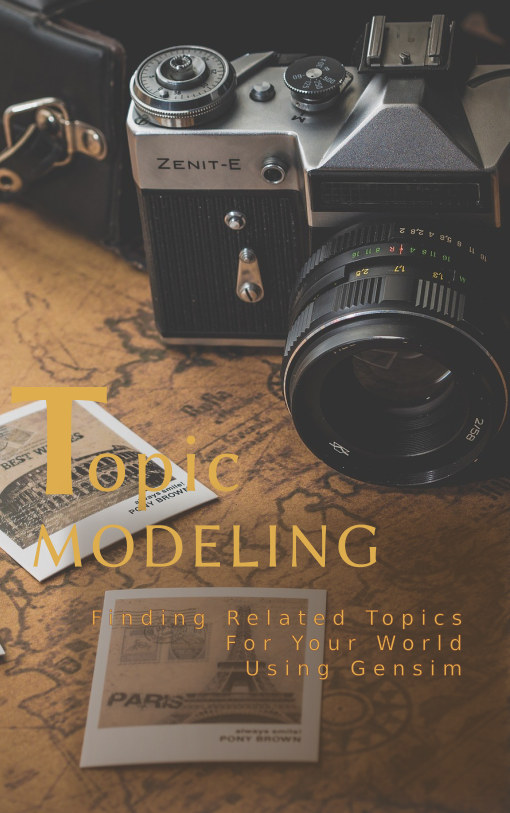
\includegraphics[width=\paperwidth]{./media/images/topic_cover}
 \end{textblock*}
 \chapter{Topic Modeling\\ \small{Finding Related Topics For Your World Using Gensim}}
\label{sec:topic}
 \begin{figure*}[h]                                                           
 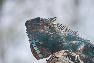
\includegraphics[width=0.95\linewidth]{./media/images/world_iguana}%
  \scriptsize{\textsc{\\topic modeling lightens} the burden of creating complete works of IF}
  \label{fig:editorial}%                                                 
\end{figure*}                                                                

\begin{quotation} 
  \noindent\color{Sepia}{\textit{\textbf{“Writing is an exploration. You start from nothing and learn as you go.”}}}\\[.5mm]
   \hfill\color{Sepia}{\small{\textendash E. L. Doctorow}}
\end{quotation} 
%\begin{abstract}
%\textbf{\emph{“In the beginning the Universe was created. This has made a lot of people very angry and been widely regarded as a bad move.”  \\ \\--- Douglas Adams}}
%\end{abstract}
\newpage
\marginnote{\href{https://www.analyticsvidhya.com/blog/2016/08/beginners-guide-to-topic-modeling-in-python/}{Shivam Bansal, Beginners Guide to Topic Modeling Modeling in Python}}[2em]
\lettrine[lines=3]{\color{BrickRed}L}{\enspace et's explore how to}
gain a foothold on our project's topic relationships
using\textsc{gensim}. Once you've determined what your work of \textsc{if} is about
it would be nice to discover what kind of related areas we can find and how all these topics tie together.

\section{relationships to diagrams} \label{sec:relations}
When we're finished, we'll be able to query the entire work of
Wikipedia about virtually any topic imaginable. Here's what a query for
\textit{Temple of Athena Nike} looks like:
\begin{lstlisting}
\$ python run_search.py
Loading Wikipedia LSI index (15-30sec.)...
   Loading LSI vectors took 2.53 seconds

Loading Wikipedia article titles...

Searching for articles similar to
'Temple of Athena Nike':
    Similarity search took 1434 ms
    Sorting took 4.40 seconds

Results:
    Temple of Athena Nike
    Temple of Poseidon at Sounion
    Temple of Hera, Olympia
    Temple of Artemis, Corfu
    Athena Alea
    Temple of Olympian Zeus, Athens
    Temple F (Selinus)
    Bassae
    ...
  \end{lstlisting}
  %Author's image
%  \begin{wrapfigure}{l}{.15\textwidth}
%    \begin{center}
%      \parbox{.15\textwidth}{
%        \includegraphics[width=.15\textwidth, keepaspectratio=true]{../images/ center_top_one_one.svg} \href{http://www.commondreams.org/author/nadia-prupis-staff-writer}{{\small{\textbf{By Nadia Prupis}}}} }
%    \end{center}
%  \end{wrapfigure} \\

  Notice that the topic modeller returns a list of related topics by order of
  relevance. The topic modeler is not a search engine\textemdash it's core
  purpose is not to \textit{match} your inquiry; its purpose
  is to return items \textit{closely related} to your inquiry. By providing
  lists of closely related topics, you can quickly map the
  results to items of exploration in your work of \textsc{if}.

  Let's take another example. First, I'll start with a known article in Wikipedia
  by looking it up
  manually.\marginnote{\href{https://en.wikipedia.org/wiki/Platonic_realism}{Base
      topic, 'Platonic Realism'}} Topic modelling is not limited to physical
constructs, and this time I'd like this time to quickly see what areas are related to
Plato's idea of realism:
\pagebreak
\begin{lstlisting}
...
Searching for articles similar to
'Platonic realism':
...
Results:
    Platonic realism
    Ontology
    Indeterminacy (philosophy)
    Theory of forms
    A priori and a posteriori
    Schema (Kant)
    Substance theory
    Nominalism
    ...
\end{lstlisting}
From here I can choose Ontology, the study of being, as a preamble to my
adventure. The interlocutor could prove that
they understand Ontology before moving to the next phase of adventure. Once they
do the room lights up to reveal a being manifested physically in the updated,
brightly lig room description.

I point a summarizer to the \emph{Platonic realism} topic:

\begin{lstlisting}
sumy lex-rank --length=5 --url https://en.wikipedia.org/wiki/Platonic_realism
\end{lstlisting}

\begin{quote}
In Platonic realism, forms are related to particulars (instances of objects and properties) in that a particular is regarded as a copy of its form.
\end{quote}
I point a summarizer to the Ontology topic:

\begin{lstlisting}
sumy lex-rank --length=5 --url https://en.wikipedia.org/wiki/ontology
\end{lstlisting}

\begin{quote}
This view allows philosophical entities other than actual entities to really exist, but not as fundamentally and primarily factual or causally efficacious; they have existence as abstractions, with reality only derived from their reference to actual entities.
\end{quote}
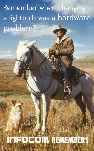
\includepdf[scale=1.01]{media/images/pepper.pdf}
And finally to the second most relevant result,
\emph{Indeterminancy\_(philosophy)} topic just for fun:
\begin{lstlisting}
sumy lex-rank --length=5 --url 'https://en.wikipedia.org/wiki/Indeterminacy_(philosophy)'
\end{lstlisting}
\begin{quote}
Science generally attempts to eliminate vague definitions, causally inert entities, and indeterminate properties, via further observation, experimentation, characterization, and explanation.
Chaos theory argues that precise prediction of the behavior of complex systems becomes impossible because of the observer's inability to gather all necessary data.
\end{quote}
\marginnote{
\label{lst:relationships}
The Graphiz graphing file \textattachfile{media/images/relationships.dot}{\color{red!50!black}{\emph{relationships.dot}}} is attached to this document (if your reader supports it) and is also \hyperlink{lst:relationships}{listed in the end notes}.
}[1em]
\pagenote[Page \pageref{lst:relationships}, Graphiz relationship graph code
listing]{\hypertarget{lst:relationships}{\lstinputlisting{media/images/relationships.dot}}
}
\noindent We can now graph the results using the Graphiz language \textemdash I see that the Indeterminacy topic mentions
'Foucault,' author of ``The Archeology of Knowlege,'' so we'll throw in
what he has to say about Indeterminacy. In a
few minutes, we get this relationship graph with the source file:
\begin{landscape}
\begin{figure*}[ht]                                                           
  \centering
  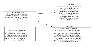
\includegraphics[width=\linewidth]{./media/images/graph}
  \caption{\textsc{entity relationship graph} graph drawn using the results of
    topic modelling.}
  \label{fig:editorial}%                                                 
\end{figure*}                                                                
\end{landscape}
\section{topic modeling preparation}
Here are the steps to create the topic modelling system:
\begin{enumerate}
  \item Downloading a complete record of all Wikipedia articles (i.e. a
    ``dump'')
  \item Converting articles to a ``big bag of words''
  \item Learning ``term-frequency–inverse document frequency'' \textsc{[tf-idf]} from bag of words
  \item Applying \textsc{tf-idf} model to all vectors
  \item Formulating a Latent Semantic Index \textsc{[lsi]} via shallow artificial neural network
    \item Applying \textsc{lsi} to all vectors
\end{enumerate}
Fortunately, a script is available \marginnote{\href{https://www.kdnuggets.com/2017/12/general-approach-preprocessing-text-data.html}{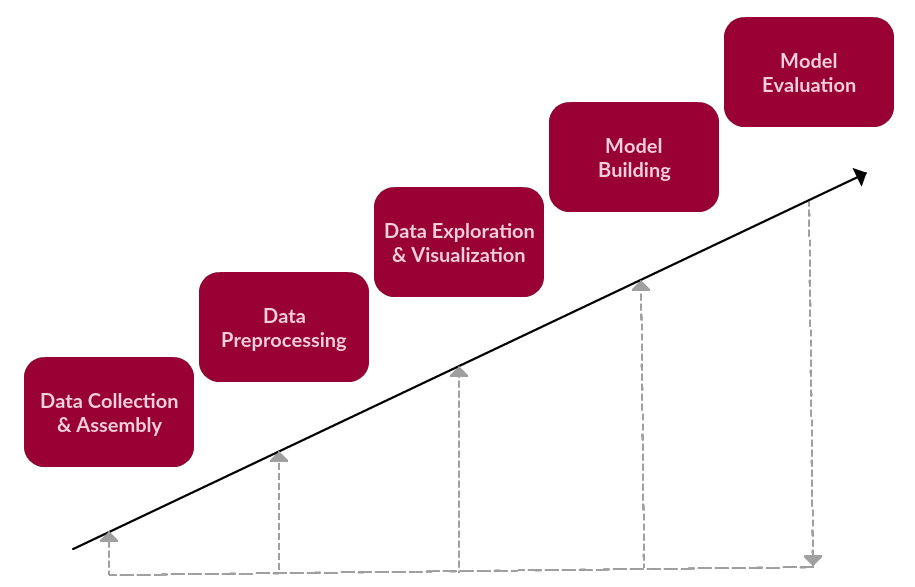
\includegraphics[width=\linewidth]{media/images/framework}\\
    Matthew Mayo, ``A General Approach to Preprocessing Text Data''}} that performs all these steps for you. Once
you've installed the necessary requirements to your system (outlined below)
you'll be ready to run the topic modeling queries as shown beginning on page
\pageref{sec:relations}. For effective topic modelling you needn't know the
details of the process.

\subsection{installing prerequisites}
\textsc{gensim} requires \textsc{python, numpy, scipy, six, and smart\_open} to run.
Fortunately, either your operating system has a pre\textendash defined package
to install that will install all these dependencies for you or \textsc{python}'s
internal \textsc{pip} installation system will install the required dependencies
for you.

Installing \marginnote{\href{https://radimrehurek.com/gensim/install.html}{\textsc{gensim} quick install guide}}[2em] from your operating system's package manager is the preferred route; it will avoid conflicts down the road. On Arch Linux, for example, the command to install Gensim through \textsc{yaourt} is:
\begin{lstlisting}
  yaourt gensim
\end{lstlisting}

\marginnote{\href{https://github.com/BurntSushi/nfldb/wiki/Python-&-pip-Windows-installation}{\textsc{python} \& \textsc{pip} Windows installation guide}}[1em]
If your system does not have a defined package for \textsc{gensim} simply
install \textsc{python} and \textsc{pip}. From there, install \textsc{gensim}
using \textsc{pip}.

If you have to install \textsc{gensim} through \textsc{pip}\textemdash as slightly
preferred in my opinion because \textsc{pip} generally provides recent versions\textemdash then
\textsc{gensim} may be installed by executing:

\begin{lstlisting}
pip install --upgrade gensim
\end{lstlisting}
\subsection{good citizenry: downloading wikipedia}
Now that \textsc{gensim} and its pre\textendash requisites are installed, we can
use these tools to download \& prepare the Wikipedia article dump
for use.

The Wikipedia article dump is big, taking around 15\textsc{gb} and growing. The
preferred way to download the dump is through a torrent file. Torrent downloads
reduce the load on a server by spreading the bandwidth use across multiple servers. The
second\textendash most preferred way is to download the dump from a Wikipedia mirror. The least
preferred way is to download the dump from Wikipedia's server proper.

Wikipedia dump file names are in the form:
\begin{lstlisting}
  enwiki-[latest]-pages-articles.xml
  \end{lstlisting}
Download the latest torrent file ({\small enwiki-20170820-pages-articles.xml.bz2} as of
this writing) to your normal download directory.

Fire up your torrent client,
\marginnote{\href{https://harbhag.wordpress.com/2010/06/30/tutorial-using-rtorrent-on-linux-like-a-pro/}{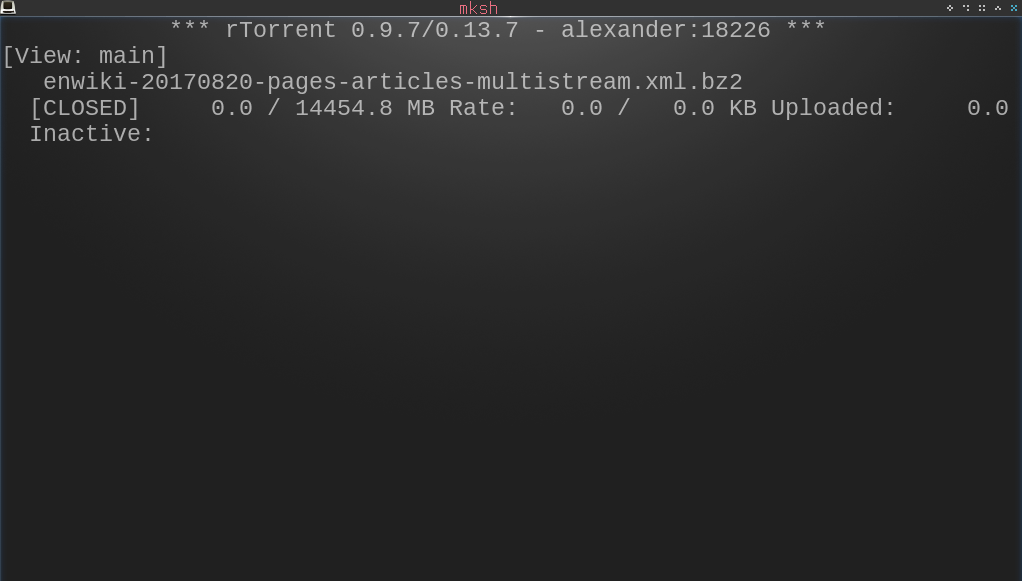
\includegraphics[width=\linewidth]{media/images/rtorrent}\\ \textsc{rtorrent}
  installation and use guide}} or double-click the torrent file you just
downloaded, and initiate the torrent download process. I personally used the
terminal\textendash based \textsc{rtorrent} but any torrent client will do. Be
patient; the Wikipedia dump is a large download and will take time to finish, even if your system is connected to fiber\textendash optic lines.
\subsection{downloading from a mirror}
Alternatively, you can download the dump from a
mirror.\marginnote{\href{https://dumps.wikimedia.org/mirrors.html}{Wikipedia
    Mirror List}}[2em] These are generally \textsc{ftp} sites. The key to finding the file you want is to navagate to the \textit{enwiki} subdirectory.
An example \textsc{url} looks like this:
\begin{lstlisting}
http://ftp.acc.umu.se/mirror/wikimedia.org/dumps/enwiki/20180901/enwiki-20180901-pages-articles.xml.bz2
\end{lstlisting}
Once you've selected the appropriate file, click the link and download as you normal.

\subsection{installing wiki\textendash sim\textendash search} \label{sec:wikisim}
\textsc{wiki-sim-search} is a python script \marginnote{\href{https://github.com/chrisjmccormick/wiki-sim-search}{\textsc{wiki\textendash sim \textendash search} Github repository, including instructions for use}}
that automatically processes the
Wikimedia articles into forms usable for topic modeling with \textsc{gensim}. To
install \textsc{wiki-sim-search} you can either download the zip file or project's
repository using \textsc{git}. 

Once \textsc{wiki-sim-search} is cloned or decompressed, copy (or move) the
\texttt{\small{enwiki-[latest]-pages-articles.xml.bz2}} to the \texttt{data} directory
of the project.

Once the Wikipedia articles are in place, run this to process the Wikipedia dump:
\begin{lstlisting}
python make_wikicorpus.py
\end{lstlisting}
It will take roughly 12 hours on an
\textsc{intel i7}. The process, at least on \textsc{linux}, will not seem to be doing
anything. Be patient\ldots if you see the cursor just blinking when the program
hasn't returned an error it is running and should finish. The output will look
similiar to this:
\begin{lstlisting}
Parsing Wikipedia to build Dictionary...
    Building dictionary took 3:05
    8746676 unique tokens before pruning.

Converting to bag of words...
    Conversion to bag-of-words took 3:47

Learning tf-idf model from data...
    Building tf-idf model took 0:47
     
Applying tf-idf model to all vectors...
    Applying tf-idf model took 1:40

Learning LSI model from the tf-idf vectors...
    Building LSI model took 2:07

Applying LSI model to all vectors...
    Applying LSI model took 2:00
\end{lstlisting}
You may get a print statement error immediately after running
\textsc{make\_wikicorpus.py} like this:
\marginnote{\href{https://docs.python.org/3/whatsnew/3.0.html\#print-is-a-function}{Changed print statement in Python 3.0}}[2em]
\begin{lstlisting}
  File "make_wikicorpus.py", line 80
    print 'Parsing Wikipedia to build Dictionary...'
SyntaxError: invalid syntax
\end{lstlisting}
This error occurs when you are running the latest version of python. Go into the
\texttt{make\_wikicorpus.py} file and add parenthesis to every print statement.
For example, change the print statement from this:
\begin{lstlisting} 
  print 'Parsing Wikipedia to build Dictionary...'
\end{lstlisting}
To this:
\begin{lstlisting}
  print ('Parsing Wikipedia to build Dictionary...')
\end{lstlisting}
\marginnote{\href{https://nlpforhackers.io/topic-modeling/}{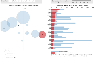
\includegraphics[width=\linewidth]{media/images/gensim_graph}\\
    Topic Modeling with \textsc{gensim} affords several ways to find and
    analyise topics and key word relationships}
} Adding parentheses to print statements also applies to the other search functions: \textsc{simsearch.py}, \textsc{keysearch.py}, and \textsc{searchwithwimwearch.py}.

Once the \textsc{make\_wikicorpus.py} function finishes you'll be ready to run
topic modeling as described at the beginning of this article. To search for a
specific topic, change the \textsc{query\_title} variable in line 29 of the
\textsc{run\_search.py} file to your topic of choice.

For example, change line 29 from this:
\begin{lstlisting}
query_title = 'Topic model'
\end{lstlisting}
To this:
\begin{lstlisting}
query_title = 'Platonic realism'
\end{lstlisting}
The ``trick'' is to search for Wikipedia articles titles proper using case
sensitive queries. To run the search again on one of the results, copy \&
paste the result and modify \textsc{run\_search.py}'s \texttt{query\_title}
variable.

Here you have it\textemdash a method for quickly pulling in topic relationships
for whatever your project calls for. By using Wikipedia as a base you are
pulling from a large ``real\textemdash world'' body of information. Even if you
model your topics loosely against the wikipedia corpus (perhaps ``Josh Wayne'' in your story is
closely modeled after ``John Wayne''), your stories
will ``feel'' authentic because they are based on authentic sources.
% \chapter*{}
% \begin{textblock*}{70.9mm}(0mm,0mm)
% \includegraphics[width=\paperwidth]{./media/images/planning_if.png}
% \end{textblock*}

%\chapter{Sketching Your Reality \\ \small{Tips For Authoring}}
%\input{./article_four.tex}

\chapter*{}
\begin{textblock*}{70.9mm}(0mm,0mm)
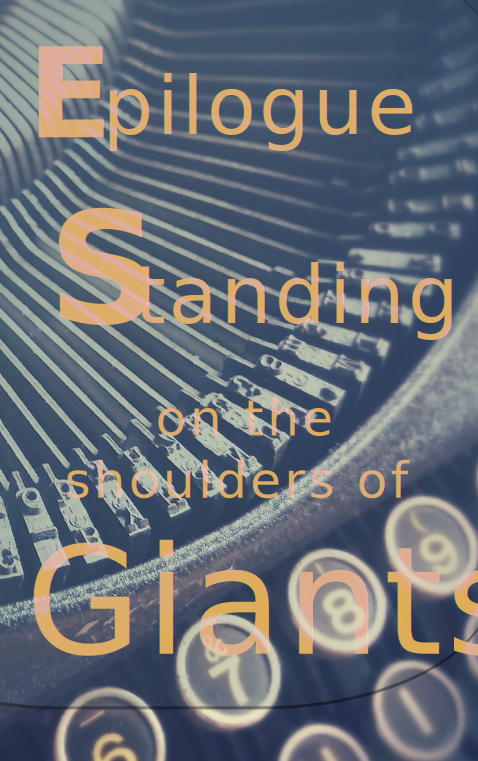
\includegraphics[width=\paperwidth]{./media/images/type}
\end{textblock*}

\chapter{Epilogue\\ \small{Standing On The Shoulders of Giants}}
\label{ch:epilogue}
\begin{figure*}[h]                                                           
 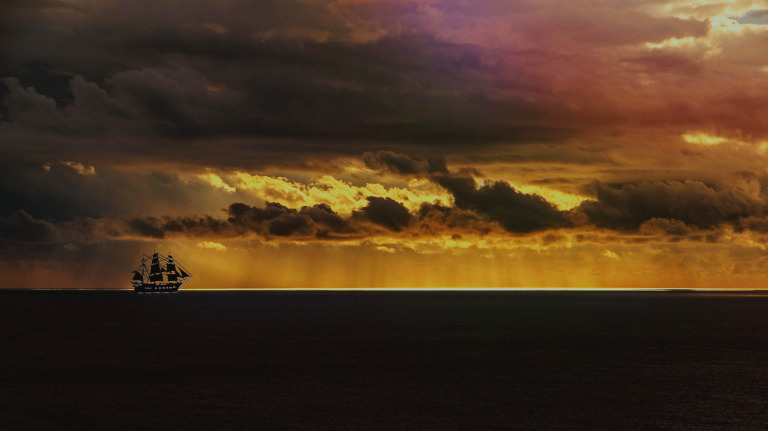
\includegraphics[width=\linewidth]{./media/images/boat}%
  \small{\textsc{\\ Peter M.J. Gross's} editing made this issue of
    \textsc{Discoverer's Digest} a much better work than it otherwise would be;
    he helped navigate my way to publishing this issue.}
  \label{fig:boat}%                                                 
\end{figure*}                                                                
\begin{quotation} 
\noindent\color{Sepia}{\small{\textit{\textbf{“Talent is a flame. Genius is
        a fire.” }}}}\\[2mm]
   \hfill\color{Sepia}{\scriptsize{\textendash Bernard Williams}}
\end{quotation} 

\section{peter m.j. gross: they don't come better}
\lettrine[lines=3]{\color{BrickRed}I}{\enspace} want to thank \textit{Peter M.J. Gross} for his fantastic work editing this
edition. To give the credit he deserves will sound trite and woefully inadequate
at the same time. Peter is a man who's thoroughness, understanding, and
relentless pursuit of quality are second to none.

By the way, Peter doesn't know I'm writing this \textit{thanks} here so if there are any
errors or awkward grammar the fault is fully my own.

\noindent Thank you, Peter.


\section{coming up}
The next issue of \textit{Discoverer's Digest} covers the results of this year's
\textsc{IF Comp} results and possibly an interview from one or two of the authors.

Covered also will be more mapping techniques and a guide for
\textsc{gps}\textendash enabled \textsc{if}.

See you next time! \\ \\

\noindent Fair Winds, \\ \\

\noindent\textsc{\href{mailto:cooper@discdigest.xyz}{D. Cooper Stevenson}}



%\noindent \href{mailto:cooper@cooper.stevenson.name}{\textsc{D. Cooper Stevenson}} 



%\chapter*{}
%\begin{textblock*}{70.9mm}(0mm,0mm)
%\includegraphics[width=\paperwidth]{./media/images/engaged}
%\end{textblock*}
%\chapter{IF In The Real World \\ \small{GPS-Enabled Adventures for Exploration}}
%\label{chap:real_world}
%\input{./article_three.tex}


% Going to Canon beach to take pictures
% - Getting back after dark

% bored waiting me to take picture of valley farm

% print page notes
\printpagenotes
\end{document}
% Author's Margin Credit
% \marginnote{\includegraphics[width=\linewidth]{/tmp/felice}\href{https://en.wikipedia.org/wiki/Republic_(Plato)}{\\\\By Felicity Banks}}

% Author's Bio
% \begin{wrapfigure}{l}{.25\textwidth}
%   \vspace{-20pt}
%   \begin{center}
%      \includegraphics[width=0.25\textwidth]{/tmp/felice}
%      \caption*{\href{http://cooper.stevenson.name}{\textit{Felicity Banks}}}
%      % } % end parbox
%     \end{center}
%  \end{wrapfigure} 
%\noindent \textit{Banks’ evocation, and then subversion and manipulation, of small details of Australian colonial history is clever and got me checking (historical) names and details on more than one occasion. The story’s action is fast-paced & drives the plot forward with a precision akin to the machinery it embraces.} \\ \\

